
% this file is called up by thesis.tex
% content in this file will be fed into the main document

%: ----------------------- introduction file header -----------------------
\chapter{The Divisor and Picard schemes}\label{chap:relative_Pic_and_Div}

%: ----------------------- paths to graphics ------------------------

% change according to folder and file names
\ifpdf
    \graphicspath{{figures/}{figures/}{figures/}}
\else
    \graphicspath{{figures/}{figures/}}
\fi

% ----------------------------------------------------------------------
%: ----------------------- introduction content ----------------------- 
% ----------------------------------------------------------------------
%: ----------------------- HELP: latex document organisation
% the commands below help you to subdivide and organise your thesis
%    \chapter{}       = level 1, top level
%    \section{}       = level 2
%    \subsection{}    = level 3
%    \subsubsection{} = level 4
% note that everything after the percentage sign is hidden from output


\nocite{*}


In the first part of this Chapter we will introduce the relative Divisor and Picard functors which, respectively, map a scheme $T$ to flat families of effective Cartier divisors and to families of line bundles with rigidification parametrised by $T$. 
The representability of such functors -- achieved under some particular assumptions -- gives rise to scheme structures for the sets of divisors and line bundles on the curve $X$ and, further, to two universal objects which will be fundamental for the rest of our discussion: the universal divisor $\Delta$ and the universal line bundle $\scL$.\\
Next, exploiting the obtained scheme structure for $\EDiv_X$ and $\Pic_X$, we will compute their tangent spaces. 
It is interesting to observe that the tangent space at a closed point $D$ of the Divisor scheme is naturally isomorphic to the cohomology group $H^0(D)_D$ arising from the sheaf-cohomology of the line bundle $\OXD$ and that, moreover, the tangent space of the Picard scheme at any closed point is simply isomorphic to $H^1(\OX)$ -- the space of first order deformations of line bundles.
This cohomological point of view leads to a description of the \AJJ map by means of the coboundary morphism 
$$ \delta_D : H^0(D)_D \tolong H^1(\OX) $$
appearing in the long cohomology sequence of $\OXD$, from which one realises that the study of linear series is deeply related to the sheaf-cohomology of the curve.\\
Finally, building on the above idea, we will achieve a global cohomological description of the tangent sheaves $T\EDiv_X$ and $T\Pic_X$ --
this is where the universal objects start to reveal their crucial role. In fact, the formal replacement of $D$ by the universal divisor $\Delta$ allows to produce a long cohomology sequence containing the locally-free sheaves $\pi_* \calO_{\Delta}(\Delta)$ and $R^1 \pi_* \calO_Z$, which we will show to be isomorphic to the tangent sheaves of $\EDiv_X$ and $\Pic_X$, respectively. 
Moreover, the \emph{global} coboundary morphism 
$$ \delta: \pi_* \calO_{\Delta}(\Delta) \tolong R^1 \pi_* \calO_Z$$
appearing in the cohomology sequence can be identified with the tangent morphism of sheaves $Tu$, thus giving a global cohomological way to describe the degeneracy loci of the \AJJ map which will be exploited in the next Chapter. 

\section{Working assumptions}\label{sec:assumptions}
	
	Let $k$ be an algebraically closed field of any characteristic. Even though most of what follows can be defined in a more general setting, we restrict our attention to the case in which the following conditions are satisfied:
	$$
		(\star)\;
		\begin{cases}
			\; f:X\to S \text{ is quasi-compact and quasi-separated } \\
			\; f:X\to S \text{ admits a section } \eps:S\to X \\			
			\; f_*\calO_{X_T} \cong \calO_T \text{ for every $S$-scheme } T \\			
		\end{cases}
	$$
	where we abuse notation by writing $f$ for the pullback morphism $X_T\to T$ given by the fibre product. It is easy to show that conditions $(\star)$ are fulfilled in our case of interest, which is described by the following assumptions:
	\begin{assumption}
		For the rest of our discussion, let $X\to S$ be a smooth projective curve of genus $g$ over an algebraically closed field $k=\bar{k}$ and let $S=\Spec(k)$ be the trivial base scheme.
	\end{assumption}


\section{The relative Divisor functor}\label{sec:Div_functor}
	%
	Let $T$ be a scheme over $S$ and let us denote by $X_T$ the fibered product $X\times_S T$. To start, let us introduce the notion of a relative effective Cartier divisors.
	\begin{defi}
		A \textbf{relative effective Cartier divisor} on $X_T/T$ is a closed subscheme $D\subset X_T$ such that its ideal sheaf $\calO_D\subset \OX$ is invertible and the map $\ph: D\to T$ is flat.\\
		Associated to any such divisor we have a map to the natural numbers given by
		$$ \deg_D : T \to \N, \qquad t \mapsto \text{rank of } \ph_*(\calO_D) \text{ as a } \calO_{T,t} \text{ - module } $$
		and, in case of this map being constantly equal to $d\in \N$, we say that $D$ has degree $d$.\\
		The sum $D_1 + D_1$ is defined as the closed subscheme of $X$ corresponding to the sheaf of ideals $\calO_{D_1}\calO_{D_2}\subset \OX$.
	\end{defi}
	We refer to \cite[Tag 01WO]{stacks-project} for further details and for a proof of the fact that relative effective Cartier divisors are closed under the above defined sum.\\
	Based on this notion we now define the contravariant functor $\DivXS$ which maps an $S$-scheme $T$ to the set of families of divisors parametrized by $T$.
	\begin{defi}
		We define the \textbf{relative effective Cartier divisors functor} by
		$$ \DivXS:\Sch_S^{op} \to \Set, \quad T \mapsto \set{ \text{ Relative effective Cartier divisors} \text{ on } X_T/T }. $$
		and the action on morphism by sending an $S$-map $T'\overset{f}\to T$ to the pullback $(1_X\times f)^*$.\\ 
		Moreover, for every $d\in \N$ define the subfunctors $\DivXS^d:\Sch_S \to \Set$ by restricting to divisors of degree $d$.
	\end{defi}
	\begin{rema}
		Notice that composition of morphisms is obviously respected and, further, the flatness of $D\to T$ ensures that the pullback $(1_X\times f)^*D$ is a relative effective Cartier divisor on $X_{T'}/T'$. Hence we see that $\DivXS$ is in fact a (contravariant) functor \\
		Further one can show that, if $\DivXS$ is representable by a scheme $\EDiv_X$, then the subfunctors $\DivXS^d$ are representable by open and closed subschemes $\Dd$ which form a disjoint cover of $\EDiv_X$ -- see Exercise 3.8 of \cite{PICARD} for details.
	\end{rema}
	\begin{notation}
		In the following we will abuse notation by simply writing $f^*$ instead of $(1_X\times f)^*$ , whenever the meaning is clear from the context and no confusion arises.
	\end{notation}
	Under reasonable hypothesis on $X\to S$, the relative Divisor functor turns out to be representable, the representing scheme being an open subscheme of the Hilbert scheme.
	\begin{theo}\label{thm:div_representable}
		If the structure morphism $f:X\to S$ is projective and flat, then the functor $\DivXS$ is representable by an open subscheme of the Hilbert scheme.
	\end{theo}
	\begin{proof}
		A proof can be found for instance in \cite{PICARD} -- see Theorem 3.7.
	\end{proof}
	Therefore under our assumptions -- $X$ a projective curve and $S=\Spec(k)$ -- the relative Divisor functor is representable.\\	

\section{The relative Picard functor}\label{sec:Pic_functor}
	
	We now want to define a relative Picard functor, which extends the concept \emph{Picard group} to flat families of line bundles parametrized by any $S$-scheme $T$. But let us first recall how the classical Picard group is defined:
	\begin{defi}
		Let $X$ be a scheme over a field $k$. We define the \textbf{Picard group} of $X$ as the as the sheaf cohomology group
		$$ \Pic(X) := H^1(X, \OX^*) $$
	\end{defi}
	There are subtle issues involved in the definition of the relative Picard functor and one needs to be careful. A naive definition could be of the form
	$$ T \mapsto \Pic(X_T)/\Pic(T) $$
	but this does not lead to a representable functor, as one can see it only defines a \emph{pre}sheaf with respect to both the \'etale and flat topologies. 
	To solve this problem and hope for a representable Picard functor, one could define it as the sheafification of the above naive one, with respect to a reasonable Grothendieck topology on the category $\Sch_S$. Another strategy, which leads to the same result but is conceptually more transparent, is to get rid of the automorphisms of the objects -- families of line bundles -- we want to parametrize with our functor. 
	We will adopt this latter approach, thus restricting our attention to the class of rigidified line bundles which we now introduce.
	\begin{defi}
		Let $f:Y\to B$ be a scheme, $\eps:B\to Y$ a section of $f$ and $L$ a line bundle over $Y$.
		A \textbf{rigidification of $L$ along} $\eps$ is an isomorphism $\al: \eps^*L \toiso \calO_B $.
		We define a \textbf{rigidified line bundle} on $Y/B$ to be a pair $(L,\al)$ consisting of a line bundle on $Y$ together with a rigidification along $\eps$.
	\end{defi}
	\begin{comment}
		A \textbf{rigidified line bundle} on $X/T$ is a line bundle $L\to X_T$ together with a rigidification $\al: \eps_T^*L \toiso \calO_T $ along $\eps_T$, where $\eps_T:T\to X_T$ is the section of $X_T\to T$ induced by a given section $\eps:S\to X$.
	\end{comment}
	One can show that, under our hypothesis, any such line bundle can be written in the form $\calO(D)$ for an effective Cartier divisor $D$ on $Y/B$. Thus we define the \textbf{degree} of a rigidified line bundle $(L,\al)$ to be the degree of the corresponding divisor.\\

	Going back to our situation $(\star)$ of a scheme $f:X\to S$ with a section $\eps:S\to X$ at our disposal, for every $T\in \Sch_S$ there is a canonical way to rigidify line bundles on $X_T/T$ along the induced section $\eps_T$ -- which by abuse of notation we will also denote by $\eps$. 

	\begin{equation*}
	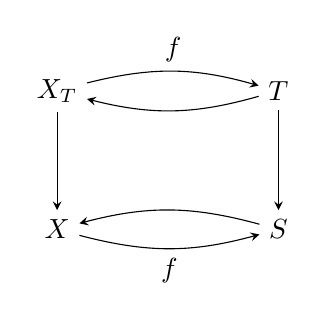
\begin{tikzpicture}[node distance=5em, auto] %SQUARE
		\node (A) 															{$X_T$};
		\node (B) 	[right of=A, xshift=3em]		{$T$};
	  \node (C) 	[below of=A] 								{$X$};
	  \node (D) 	[right of=C, xshift=3em] 		{$S$};
	  %
	  \draw[-stealth, bend left=15, looseness=1]						(A)		to node {$f$} 			(B);
	  \draw[-stealth, bend left=15, looseness=1]						(B)		to node {$\eps$} 	(A);
	  \draw[-stealth]																				(A)		to node {} (C);
	  \draw[-stealth]																				(B)		to node {} (D);
	  \draw[-stealth, bend right=15, looseness=1, swap]			(D)		to node {$\eps$}		(C);
	  \draw[-stealth, bend right=15, looseness=1, swap]			(C)		to node {$f$} 			(D);
	\end{tikzpicture}
	\end{equation*}

	In fact, given a line bundle $M$ over $X_T$, one can obtain a line bundle $(L,\al)$ with rigidification along $\eps$ by setting
	$$ L:= M\otimes f^* \eps^* M^{-1} . $$
	Indeed, recalling that by definition of section $f\circ\eps \equiv 1$, we find that
	$$ 
	\eps^* L 
	= 
	\eps^*M\otimes \eps^* f^* \eps^* M^{-1} 
	= 
	\eps^*M\otimes (f\circ\eps)^* \eps^* M^{-1}
	=
	\eps^* (M\otimes M^{-1})
	=
	\calO_T  
	$$
	as desired.
	The key feature of rigidified line bundles is that they do not admit nontrivial automorphisms, as we show in Proposition \ref{prop:rigid} of Appendix A.\\

	We are now ready to define the relative Picard functor:
	\begin{defi}
		We define the \textbf{relative Picard functor} by the assignment
		$$ \PicXS:\Sch_S^{{op}} \to \Ab, \qquad T \mapsto \set{ \text{Rigidified line bundles}\text{ on } X_T/T } $$
		and the action on morphism by sending an $S$-map $T'\overset{f}\to T$ to the pullback $(1_X\times f)^*$.\\ 
		Moreover, for every $d\in \N$, we define the subfunctors $\PicXS^d:\Sch_S \to \Set$ by restricting to line bundles of degree $d$.
	\end{defi}
	\begin{rema}
		Notice that composition of morphisms is obviously respected and, further, it is a well known fact that line bundles are stable under pullbacks. Hence we see that $\PicXS$ is in fact a (contravariant) functor.
	\end{rema}	
	It can be shown (see for instance Section 8.1 of \cite{BOSCH}) that conditions $(\star)$ imply the representability of $\PicXS$ and, moreover, that for every $S$-scheme $T$ there is a natural isomorphism
	\begin{equation}\label{eq:PicXS}
		\PicXS(T) \;\cong\; \Pic(X_T) / \operatorname \Pic(T)
	\end{equation}

\section{Universal divisor and universal line bundle}
	%
	As remarked above, under our hypothesis Theorem \ref{thm:div_representable} applies, therefore $\DivXS^d$ is representable and we will denote the representing $S$-scheme by $\Dd$, which is unique up to unique isomorphism. For $\Dd$ to be the representing scheme it means that there are canonical isomorphisms
	$$ \DivXS(T) \;\cong\; \HomS(T,\Dd), \quad \forall \;T\in \Sch_S $$
	and a universal object $\Delta \in \DivXS(\Dd)$ with the property that to every morphism $f\in \HomS(T,\Dd)$ corresponds a unique $D\in \DivXS(T)$ given as the pullback $f^*(\Delta)$ of $\Delta$ via $f$. This is the universal property of $\Delta$. 
	Notice that there is a bijection between the set of closed points of $\Dd$ and the set of effective divisors of degree $d$ on $X$. In particular with $T=S$, for any divisor $D\in \Dd$ there is a unique canonical $S$-map $f:S\into\Dd$ such that $f^*(\Delta) = D$.\\

	The same reasoning applies to line bundles: as soon as $\PicXS^d$ is representable we get a representing $S$-scheme $\Pd$ unique up to unique isomorphism (whose points are line bundles of degree $d$ on $X/S$) and a universal line bundle $\scL \in \PicXS(\Pd)$. Notice that, under our hypothesis, the relative Picard functor $\PicXS$ is representable and identification $\eqref{eq:PicXS}$ holds.\\

	Due to their importance in the rest of our discussion, we summarize below the nature of the universal objects we just obtained, in a concise fashion: 
	\begin{notation}
		The above universal objects are denoted by
		$$
			\begin{array}{ l c l }
				\Delta\;\subset\; X\times \Dd \qquad &\leadsto& \textbf{ Universal divisor }
				\\\\
				\scL \longrightarrow X\times \Pd \qquad &\leadsto& \textbf{ Universal line bundle }
			\end{array}
		$$
	\end{notation}\vspace{1em}
	It is interesting to notice that, as we will show in the next sections, these universal objects can be used to describe the tangent sheaves of the Divisor and Picard schemes.\vspace{1em}

\section{Tangent spaces of $\Dd$ and $\Pd$ }\label{sec:tgnt_spaces}
	%
	Within the categorical setting introduced in the previous Sections, the Abel-Jacobi map can be seen as a natural transformation of functors between $\DivXS$ and $\PicXS$.
	\begin{defi}
		We define the Abel-Jacobi map (also known as the Albanese map) as the natural transformation of functors
		$$ u: \DivXS \to \PicXS, \qquad \scr{D} \mapsto \calO(\scr{D}).$$
	\end{defi}
	For every $d\in \N$ the classical Abel-Jacobi map induces a morphism in the category of schemes over $S$, between the representing schemes
	$$ u :  \Dd \to \Pd, \qquad D \mapsto \OXD $$
	and, in order to study its tangent map at a closed point $D\in \Dd$
	$$ \TDu : T_D \Dd \to T_{u(D)} \Pd \,, $$
	we should, first of all, understand the above tangent spaces. A very useful tool for this purpose is the ring of the dual numbers $ k_\eps = k[\eps]/\eps^2 $ and the associated fibred product 
	$$ X_\eps := X \underset{{S}}\times {\Spec(k_\eps)}. $$ 
	Moreover, for any $k$-scheme $P$ with a rational point $e$, denote by $P(k_\eps)_e$ the set of all $k$-maps from the \emph{free tangent vector} $\Spec(k_\eps)$ to $P$ which are supported at $e$. \\

	In this situation Lemma \ref{lemm:tng_sch} of Appendix A shows that the $k$-vector space $P(k_\eps)_e$ is in fact isomorphic to the tangent space to $P$ at the point $e$, in formula
	$$ P(k_\eps)_e \; \cong \; T_e P. $$
	Further Lemma \ref{lemm:tng_grp_sch} of Appendix A tells us that, if $P$ is a group scheme, then the tangent space at the identity element $e$ is simply given by
	$$ T_e P \;\cong\; \ker \Big( P(k_\eps) \to P(k) \Big). $$
	In order to describe the tangent space of $ \Pd$ it is useful to introduce the normal sheaf associated to a divisor, by means of the following 
	\begin{defi}
		The \textbf{normal sheaf} associated to a divisor $D\in  \Pd$ is defined as
		$$ \ODD := \OXD \otimes \calO_D. $$
		We remark that, even though $\ODD$ is a sheaf on $D$, we will often treat it as a sheaf on $X$ by implicitly pushing it forward via the natural inclusion of $D$ into $X$. 
	\end{defi}
	\begin{notation}
		With the aim of making our notation lighter, we will often write 
		$$ H^i(D)_{D} \equiv H^i(X,\ODD)$$ 
		for the $i$-th cohomology group of the normal sheaf.
	\end{notation}
	\begin{rema}\label{rema:div_ses}
		The ideal sheaf of $\calO_D$ is $\OX(-D)$, so we have a natural \ses
		$$ \SES{\OX(-D)}{\OX}{\calO_D} $$
		and, since tensoring with the invertible sheaf $\OXD$ leaves the sequence exact, we get
		$$ \SES{\OX}{\OXD}{\ODD}. $$			
	\end{rema}
	The following proposition shows that the normal sheaf $\ODD$ is the house of the infinitesimal deformations of a divisor $D$, so that the tangent space of $\Dd$ at $D$ is just its space of global sections $\HDD$.
	\begin{prop}\label{prop:tgn_div}
		Let $D$ be a closed point of $ \Dd$. We have an isomorphism of vector spaces
		$$ T_D \Dd \cong \HDD. $$
	\end{prop}
	\begin{proof}
		From Lemma \ref{lemm:tng_sch} of Appendix A we know that the tangent space $T_D \Dd = T_D\DivXS(k)$ coincides with $ \DivXS(k_\eps)_D$, which can be described as the vector space
		
		$$ 
		V = \set{\parbox{8.2cm}{
		Relative effective Cartier divisors on $X_\eps / k_\eps$ 
		whose pull-back to the closed fibre $X\subset X_\eps$ is $D$.
		}}
		\vspace{0.5em}
		$$

		Let $G_i \in H^0(U_i,\OX(-D)) $ be local equations for $D$ over an open cover $U_i$. Then an element of $V$ has local equations
		$$ F_i = G_i + \eps H_i, \qquad H_i \in H^0(U_i,\OX) $$
		satisfying the glueing condition $F_i = (\text{unit})\cdot F_j$ on $U_{i,j}$. Equivalently, such conditions can be expressed as
		$$ G_i + \eps H_i = (a_{i,j} + \eps b_{i,j})\cdot (G_j + \eps H_j) $$
		for some $b_{i,j} \in H^0(U_{i,j},\OX)$ and $ a_{i,j} \in H^0(U_{i,j},\OX^*)$, which implies that
		$$ G_i = a_{i,j} G_j \AND H_i = a_{i,j} H_j + b_{i,j}G_j. $$
		It follows that the assignment $F_i \mapsto H_i/G_i$ is well-defined, since the identity
		$$ \frac{H_i}{G_i}-\frac{H_j}{G_j} = b_{i,j}\cdot a_{j,i} $$
		ensures that $\{H_i/G_i \} $ glues to a global section of $\ODD$. It is easy to check that this gives a bijections of vector spaces.
	\end{proof}
	We now turn to the tangent space of the Picard scheme, which actually admits a simpler description.
	\begin{prop}\label{prop:tgn_pic}
		Let $L$ be a closed point of $ \Pd$ and assume conditions $(\star)$ of Section \ref{sec:assumptions} are met. Then we have an isomorphism of vector spaces
		$$ T_L \Pd \cong H^1(\calO_X). $$
	\end{prop}
	\begin{proof}
		First of all notice that $\Pic = \sqcup_{d\in \N}\Pd$ is a group scheme, therefore the tangent space at every point $L$ is canonically isomorphic to the tangent space at the identity element $ 0\in \Pic^0_X = \PicXS^0(k)$.
		Hence, from Lemma \ref{lemm:tng_grp_sch} of Appendix A we know what we are looking for: the kernel of the map $ \PicXS(k_\eps)\to  \PicXS(k)$. In order to compute it, consider the truncated exponential sequence
		$$ \SES{\OX}{\calO_{X_\eps}^*}{\OX^*}, $$
		where the first map is the exponentiation $e: f\mapsto 1+\eps f$. Notice that this map enjoys the key property of the classical exponential, as we have 
		$$ e(f + g) = 1+\eps(f+g) = (1+\eps f)\cdot(1+\eps g) = e(f) \cdot e(g) $$
		so that its name is justified. The above sequence splits using the natural inclusion of $\OX^*$ into $\calO_{X_\eps}^*$, so we obtain a \ses in cohomology of degree $1$
		$$ \SES{H^1(\OX)}{H^1(\calO_{X_\eps}^*)}{H^1(\OX^*)}. $$
		Now, the fact that conditions $(\star)$ are satisfied implies that the natural identification \eqref{eq:PicXS} holds, thus giving isomorphisms
		$$ \PicXS(k) \cong \Pic(X) = H^1(\OX^*) \AND \PicXS(k) \cong \Pic(X_\eps) = H^1(\calO_{X_\eps}^*)\,. $$
		Therefore we have the following commutative diagram with exact rows, where the two vertical arrows on the right are isomorphisms and thus the same holds for the induced vertical map between the kernels.
		$$
		\begin{tikzpicture}[node distance=4em, auto]
			\node (O) 															{$0$};
			\node (A) 	[right of=O, xshift=2em]		{$H^1(\OX)$};
			\node (A2) 	[right of=A]								{$\;$};
			\node (B) 	[right of=A2]								{$H^1(\calO_{X_\eps}^*)$};
			\node (B2) 	[right of=B]								{$\;$};
		  \node (C) 	[right of=B2] 							{$H^1(\OX^*)$};
		  \node (OO) 	[right of=C, xshift=2em] 		{$0$};
		  \node (O') 	[below of=O] 								{$0$};
		  \node (A') 	[below of=A] 								{$T_0 \PicXS(k)$};
		  \node (B') 	[below of=B] 								{$ \PicXS(k_\eps)$};
		  \node (C') 	[below of=C] 								{$ \PicXS(k)$};
		  \node (OO') [below of=OO] 							{$0$};
		  \draw[-stealth] 				(O)	to node {} (A);
		  \draw[-stealth]					(A)		to node {} (B);
		  \draw[-stealth]					(B)		to node {} (C);
		  \draw[-stealth]					(C)		to node {} (OO);
		  \draw[-stealth]					(O')	to node {} (A');
		  \draw[-stealth]					(A')	to node {} (B');
		  \draw[-stealth]					(B')	to node {} (C');
		  \draw[-stealth]					(C')	to node {} (OO');
		  \draw[-stealth][dashed]	(A)	to node {} (A');
		  \draw[-stealth]					(B)		to node {} (B');
		  \draw[-stealth]					(C)		to node {} (C');
		\end{tikzpicture}
		$$
		Finally, one can easily check that the above dashed isomorphism is in fact an isomorphism of vector spaces.
	\end{proof}

\section{Tangent bundles of $\Dd$ and $\Pd$ }
	In the last section we gave an entirely cohomological description of the tangent spaces of both $\Dd$ and $\Pd$. We will now show that we can actually do much better, giving a cohomological description for the tangent \emph{sheaves} of those varieties, thus achieving a global analogue of the identifications obtained, fiberwise, in the last section. \\
	We start with a Lemma showing that the sheaves we are interested in are locally-free.

	\begin{notation}
		In order to make our notation shorter, in the following we will use write simply $Z$ to denote the product $X\times \Dd$, and we will write $\pi:Z\to \Dd$ for the natural projection on the second factor. 
	\end{notation}

	\begin{defi}
		A \textbf{locally free sheaf} of rank $n$ on a scheme $Y$ is defined as an $\calO_Y$-module $\scr{F}$ that is locally a free sheaf of rank $n$. More precisely, there is an open cover $\{U_i\}$ of $Y$ such that over each $U_i$ we have an isomorphism $\scr{F}_{\mid U_i} \cong \calO_{U_i}^{\oplus n}$.
	\end{defi}

	\begin{rema}\label{rema:smoothness}
		It is a well known fact that, in our case of a smooth projective curve over an algebraically closed field, the representing schemes $\Dd$ and $\Pd$ are in fact smooth varieties in any characteristic. We do not prove these facts here but we refer to the literature -- see for instance the discussion in Chapter 5 of $\cite{PICARD}$. Therefore it follows that the tangent sheaves $T\Dd$ and $T\Pd$ are locally-free.\\
		Moreover, we remark that the quasi-coherent sheaves $\pi_* \calO_{\Delta}(\Delta)$ and $R^1\pi_*\calO_Z$ are locally-free, as will show in Proposition \ref{prop:free_pres}.\\
	\end{rema}

	Starting from the tangent sheaf of the Divisor scheme, our strategy is to pass from a single divisor $D$ to the universal divisor $\Delta$, making the formal replacement 
	$$ \HDD, \text{ vector space } \qquad \large\mapsto \qquad \pi_* \calO_{\Delta}(\Delta), \text{ locally free sheaf }$$
	
	\begin{prop}
		There is a canonical isomorphism of sheaves $T\Dd \cong \pi_* \calO_{\Delta}(\Delta)$.
	\end{prop}
	\begin{proof}
		Let $\tilde{\pi}$ denote the restriction of $\pi:X\times\Dd\to \Dd$ to the divisor $\Delta$ and look at the diagram of the closed immersion
		$$
		\begin{tikzpicture}[node distance=4em, auto]
			\node (A) 														{$\Delta$};
			\node (B) 	[right of=A, xshift=3em]	{$X\times\Dd$};
		  \node (C) 	[below of=B] 							{$\Dd$};
		  %
		  \draw[right hook-stealth]				(A)		to node {} 								(B);
		  \draw[-stealth]									(B)		to node {$\pi$} 					(C);
		  \draw[-stealth][swap]						(A)		to node {$\tilde{\pi}$} 	(C);
		\end{tikzpicture}
		$$
		from which we readily observe that we have natural identifications
		$$ 
		\tilde{\pi}^* (T \Dd) = (\pi^* T \Dd)_{\mid_\Delta} 
		\AND 
		T (X\times\Dd)_{\mid_\Delta} = (\pi^* T\Dd)_{\mid_\Delta} \oplus (\operatorname{Pr}^*_X TX)_{\mid_\Delta} .
		$$
		Moreover, since $\calO_{\Delta}(\Delta)$ is the normal bundle of the divisor $\Delta$, there is a natural map
		$$ T(X\times \Dd) \tolong \calO_{\Delta}(\Delta) $$
		which, in light of the above identifications, gives a map from $\pi^*T\Dd $ to $ \calO_{\Delta}(\Delta)$ obtained by restriction. Therefore by the adjunction between $\pi_*$ and $\pi^*$ we find what we were looking for: a morphism		
		$$ T\Dd \tolong \pi_* \calO_{\Delta}(\Delta). $$
		As remarked in Remark \ref{rema:smoothness}, the two sheaves in question are locally free of finite rank, therefore it is sufficient to show that the above global map induces isomorphisms on each fibre. One can check that, in fact, this global morphisms restricts on every fibre to the linear map
		$$ T_D \Dd \toiso \HDD $$
		which we proved to be an isomorphism in Proposition \ref{prop:tgn_div}, thus achieving the desired conclusion.
	\end{proof}
	We now turn to the case of the Picard scheme, in which our strategy is in some sense to make the formal replacement
	$$ H^1(\OX), \text{ vector space } \qquad \large\mapsto \qquad R^1 \pi_* \calO_Z, \text{ locally free sheaf }$$
	\begin{prop}
		There is a canonical isomorphism of sheaves $u^* T\Pd \cong R^1 \pi_* \calO_Z$.
	\end{prop}
	\begin{proof}
		First of all recall from Proposition \ref{prop:tgn_pic} that we have an isomorphism
		$$ T_0 \PicXS \cong H^1(X, \OX)$$
		then notice that, since $\PicXS$ is a group variety, its tangent sheaf is constant with fibers $H^1(X, \OX)$. The same is true if we restrict to the subscheme $\Pd$, thus we see that $ T \Pd $ is the constant sheaf $\underline{H^1(X,\OX)}$ over $\Pd$. \\

		Actually, we claim that $R^1 \pi_* \calO_{Z}$ is also constant with fibers $H^1(X, \OX)$. To see this consider the base change diagram
		$$
		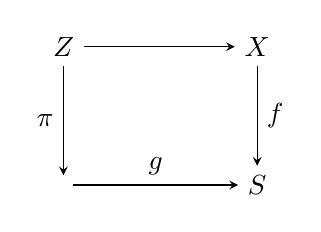
\begin{tikzpicture}[node distance=5em, auto]
			\node (A) 															{$Z$};
			\node (B) 	[right of=A, xshift=2em]		{$X$};
		  \node (C) 	[below of=A] 								{$\Dd$};
		  \node (D) 	[right of=C, xshift=2em] 		{$S$};
		  %
		  \draw[-stealth]					(A)		to node {} (B);
		  \draw[-stealth][swap]		(A)		to node {$\pi$} (C);
		  \draw[-stealth]					(B)		to node {$f$} (D);
		  \draw[-stealth]					(C)		to node {$g$} (D);
		\end{tikzpicture}
		$$
		and notice that, since we are assuming $S=\Spec(k)$, the structure morphism $f:X\to S$ is flat. Hence the above diagram describes a flat base change and thus ( use Proposition 9.3 of $\cite{HAG}$ for instance ) we get
		$$ R^1 \pi_*\calO_{Z} \cong g^* \left( R^1f_*\OX \right) \cong  g^* H^1(X,\OX), $$
		from which we deduce that $R^1\pi_* \calO_{Z}$ is the constant sheaf with fibers $H^1(X,\OX)$ over $\Dd$. Therefore it follows that $ u^* T \Pd \cong R^1 \pi_* \calO_{Z} $ .
 	\end{proof}

\section{Cohomological description of the Abel-Jacobi map}
	In this section we will achieve a purely cohomological description of the tangent map $Tu$ of the Abel-Jacobi map, first fiberwise and then globally.
	\subsection{Fiberwise description}
		In section \ref{sec:tgnt_spaces} we showed that, on every closed point $D$, the tangent morphism $\TDu$ is a linear map $\HDD\to H^1(\OX)$, which looks pretty familiar. Indeed from the natural \ses	of sheaves of Remark \ref{rema:div_ses}, i.e.
		$$ \SES{\OX}{\OXD}{\ODD} $$
		we get, observing that $H^1(X,\ODD)$ is trivial since $D$ is $0$-dimensional, the following \les in cohomology
		\begin{equation}\label{eq:abel_les}
			0\to H^0(\OX) \to H^0(D) \to \HDD \overset{\delta_D}\longrightarrow H^1(\OX) \to H^1(D) \to 0
		\end{equation}
		and we are going to show that the coboundary map $\delta_D$ can be identified with $\TDu$.
		\begin{prop}\label{prop:delta_u}
			Under the isomorphisms of Propositions \ref{prop:tgn_div} and \ref{prop:tgn_pic}, the maps $\delta_D$ and $\TDu$ can be identified.
		\end{prop}
		\begin{proof}
			We want to prove the commutativity of the following diagram
			$$
			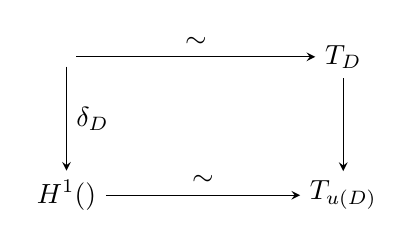
\begin{tikzpicture}[node distance=5em, auto]
				\node (A) 									{$\HDD$};
				\node (A2) 	[right of=A]		{$\;$};
				\node (B) 	[right of=A2]		{$T_D \Dd$};
			  \node (C) 	[below of=A]	 	{$H^1(\OX)$};
				\node (C2) 	[below of=A2]		{$\;$};
			  \node (D) 	[below of=B] 		{$T_{u(D)} \Pd$};
			  \draw[-stealth] 				(A)		to node {$\sim$} 				(B);
			  \draw[-stealth]					(C)		to node {$\sim$} 				(D);
			  \draw[-stealth]					(A)		to node {$\delta_D$} 	(C);
			  \draw[-stealth]					(B)		to node {$\TDu$} 			(D);
			\end{tikzpicture}
			$$
			where the lower horizontal map is the exponentiation $f\mapsto 1+\eps f$.\\
			Let $G_i$ be local equations for $D$ and $H_i/G_i$ represent a global section of $\HDD$. The coubandary map acts on it as
			$$ \delta_D\left(\frac{H_i}{G_i}\right) =  \frac{H_i}{G_i}-\frac{H_j}{G_j}. $$
			On the other hand, $H_i/G_i$ is identified with the element of $T_D \Dd$ defined by local equations $F_i = G_i + \eps H_i$ and gets mapped through $\TDu$ to the element of $T_{u(D)} \Pd$ with transition functions given by
			$$ \sigma_{i,j} = F_i / F_j. $$
			This can be expanded (here's the trick!) as
			\begin{eqnarray*}
				\sigma_{i,j} &=& (G_i + \eps H_i)/(G_j + \eps H_j) \\
				&=& G_i G_j^{-1}\cdot(1+\eps H_i/G_i)\cdot(1-\eps H_j/G_j) \\
				&=& G_i G_j^{-1}\cdot(1+\eps (H_i/G_i - H_j/G_j)).
			\end{eqnarray*}
			Now notice that $G_i G_j^{-1}$ represents a section of $\OXD$, thus we can divide them out: this just means translating $\sigma_{i,j} $ back to the origin of $ \Pd$. We are left with
			$$ 1 + \eps\left( \frac{H_i}{G_i}-\frac{H_j}{G_j} \right), $$
			which is the image under the exponential map of $\delta_D(H_i/G_i)$, as we wanted.
		\end{proof}
		We can now rewrite the \les \eqref{eq:abel_les} as
		\begin{equation}\label{eq:local_diagram}
		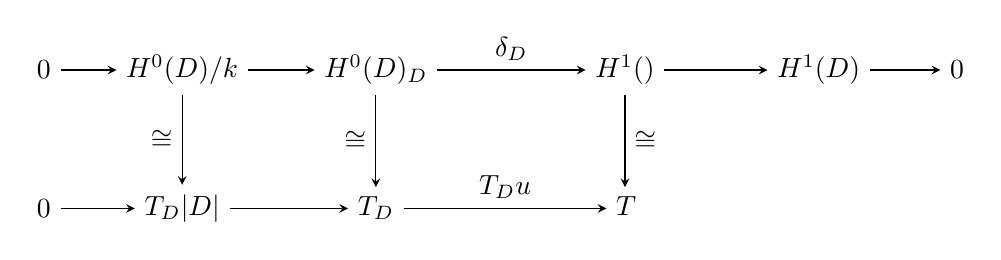
\begin{tikzpicture}[node distance=5em, auto]
			\node (O) 									{$0$};
			\node (A) 	[right of=O]		{$H^0(D)/k$};
			\node (B) 	[right of=A, xshift=2em]		{$H^0(D)_D$};
		  \node (C) 	[right of=B, xshift=4em] 		{$H^1(\OX)$};
		  \node (D) 	[right of=C, xshift=2em] 		{$H^1(D)$};
		  \node (OO) 	[right of=D] 		{$0$};
		  \node (O') 	[below of=O] 		{$0$};
			\node (A') 	[below of=A] 		{$ T_D |D|$};
		  \node (B') 	[below of=B] 		{$ T_D \Dd$};
		  \node (C') 	[below of=C] 		{$ T_{\OXD} \Pd $};
		  \node (D') 	[below of=D] 		{$\;$};
			\draw[-stealth] 				(O)		to node {} (A);
		  \draw[-stealth]					(A)		to node {} (B);
		  \draw[-stealth]					(B)		to node {$\delta_D$} (C);
		  \draw[-stealth]					(C)		to node {} (D);
			\draw[-stealth]					(D)		to node {} (OO);
			\draw[-stealth] 				(O')	to node {} (A');
		  \draw[-stealth]					(A')	to node {} (B');	  
		  \draw[-stealth]					(B')	to node {$T_D u$} (C');
		  \draw[-stealth][swap]		(A)		to node {$\cong$} (A');
		  \draw[-stealth][swap]		(B)		to node {$\cong$} (B');
		  \draw[-stealth]					(C)		to node {$\cong$} (C');
		\end{tikzpicture}
		\end{equation}	
		from which we make the following observations:
		\begin{enumerate}[i)]
			\item The dimension of the Picard scheme is bounded by $h^1(\OX)$ and equality holds \ABiff $ \Pd$ is smooth, at any point and hence everywhere. In the case of $X$ being a smooth curve of genus $g$, recall that by definition $h^1(\OX)=h^0(K)=g$;
			\item The kernel of $\TDu$ is $H^0(D)/k \cong \PP H^0(D)$, so one notices that $u$ is constant on linear series. This is the content of Abel's theorem.
		\end{enumerate}

	\subsection{Global description}

		In the last Section we showed that the tangent spaces of $\Dd$ and $\Pd$ can be seen as cohomology groups and, further, that the tangent map $\TDu$ at any point $D$ is a linear map of vector spaces. 
		We now want to make this idea global, aiming for a cohomological description of the tangent sheaves of $\Dd$ and $\Pd$ and the sheaf morphism $\Tu$. 
		To do so, we will make use of the universal divisor $\Delta$ and the universal line bundle $\scL$ to obtain two exact sequences of sheaves, which will serve as global analogues of \eqref{eq:abel_les}. 
		Moreover, we will show that the last part of these sequences are free presentations, a fact that will be of crucial importance for the definition of the moduli varieties parametrising linear series and, in general, for the rest of our discussion.\\

		\begin{defi}\label{def:Gamma}
			Choose a divisor $M = \sum_{i=1}^m P_i$ consisting of $m \geq 2g-d-1$ distinct points of $X$, then define the product divisor 
			$$\Gamma := M\times \Pd$$
		\end{defi}	


		\begin{prop}\label{prop:free_pres}
			Let $\pi : X\times \Dd \to \Dd$ and $\nu : X\times \Pd \to \Pd$ denote the natural projections on the second factor. Then the exact sequence of sheaves
			\begin{equation}\label{eq:univ_div_seq}
				\pi_* \calO_{\Delta}(\Delta)\overset{\delta}\to R^1 \pi_* \calO_Z \to R^1 \pi_* \calO_Z(\Delta) \to 0
			\end{equation}
			is a free presentation of $R^1 \pi_* \calO_Z(\Delta)$, while the exact sequence of sheaves
			\begin{equation}\label{eq:univ_lb_seq}
				\nu_{*} \scL(\Gamma)\to \nu_{*} \scL(\Gamma) / \scL \to R^1 \nu_{*} \scL \to 0
			\end{equation}		
			is a free presentation of $R^1 \nu_{*} \scL$.
		\end{prop}
		\begin{proof}
			We start by looking at the natural \ses
			\begin{equation}\label{eq:univ_div_ses}
				\SES{\calO_Z}{\calO_Z(\Delta)}{\calO_\Delta(\Delta)} 
			\end{equation}
			associated to the universal divisor, which is in some sense the global analogue of the second sequence appearing in Remark \ref{rema:div_ses}. Since $D$ is $0$-dimensional and $h^1(D_D)= 0$, Proposition \ref{prop:no_jumps} of Appendix A implies that $R^1 \pi_* \calO_{\Delta}(\Delta) = 0$, therefore the last part of the direct image sequence of \ref{eq:univ_div_ses} is given by
			$$
				\pi_* \calO_{\Delta}(\Delta)\overset{\delta}\to R^1 \pi_* \calO_Z \to R^1 \pi_* \calO_Z(\Delta) \to 0.
			$$
			As we showed in Section \ref{sec:tgnt_spaces}, for every $D\in \Dd$ the cohomology groups
			$$ H^0(X, D_D) \cong T_D \Dd \AND H^1(X, \OX) \cong T_{\OXD} \Pd $$
			are fiberwise vector spaces of dimensions $d$ and $g$. Hence Proposition \ref{prop:no_jumps} implies that $\pi_* \calO_{\Delta}(\Delta)$ is locally free of rank $d$ and that $R^1 \pi_* \calO_Z$ is locally free of rank $g$, thus showing that \eqref{eq:univ_div_seq} is in fact a \textbf{free} presentation.
			\\
			Moving towards the second sequence, notice that we have the natural \ses 
			\begin{equation}\label{eq:univ_lb_ses}
				\SES{\scL}{\scL(\Gamma)}{\scL(\Gamma)/\scL} 
			\end{equation}
			and, since by Lemma \ref{lemm:trivial_R1} of Appendix A we have $R^1 \nu_{*} \scL(\Gamma) = 0$, the corresponding direct image sequence is given by
			\begin{equation}\label{eq:univ_lb_direct_image}
				0 \to \nu_{*}\scL \to \nu_{*} \scL(\Gamma)\overset{\gamma}\tolong \nu_{*} \scL(\Gamma) / \scL \to R^1 \nu_{*} \scL \to 0 \,.
			\end{equation}
			Moreover, since for every $L\in \Pd$ the \RR implies $h^0(X, L(M)) = d+m-g+1 $, another application of Proposition \ref{prop:no_jumps} implies that  $\nu_{*} \scL(\Gamma)$ is locally free of rank $d+m-g+1$. 
			Finally, we notice that $\scL(\Gamma) / \scL$ can be seen as a line bundle on $\Gamma$, so it follows that $\nu_{*} \scL(\Gamma) / \scL$ is locally free of rank $m$, as $\nu$ restricts to a finite locally free morphism of degree $m$ on $\Gamma\subset X\times \Pd$.
		\end{proof}

		\begin{figure}[ht]
				\centering
				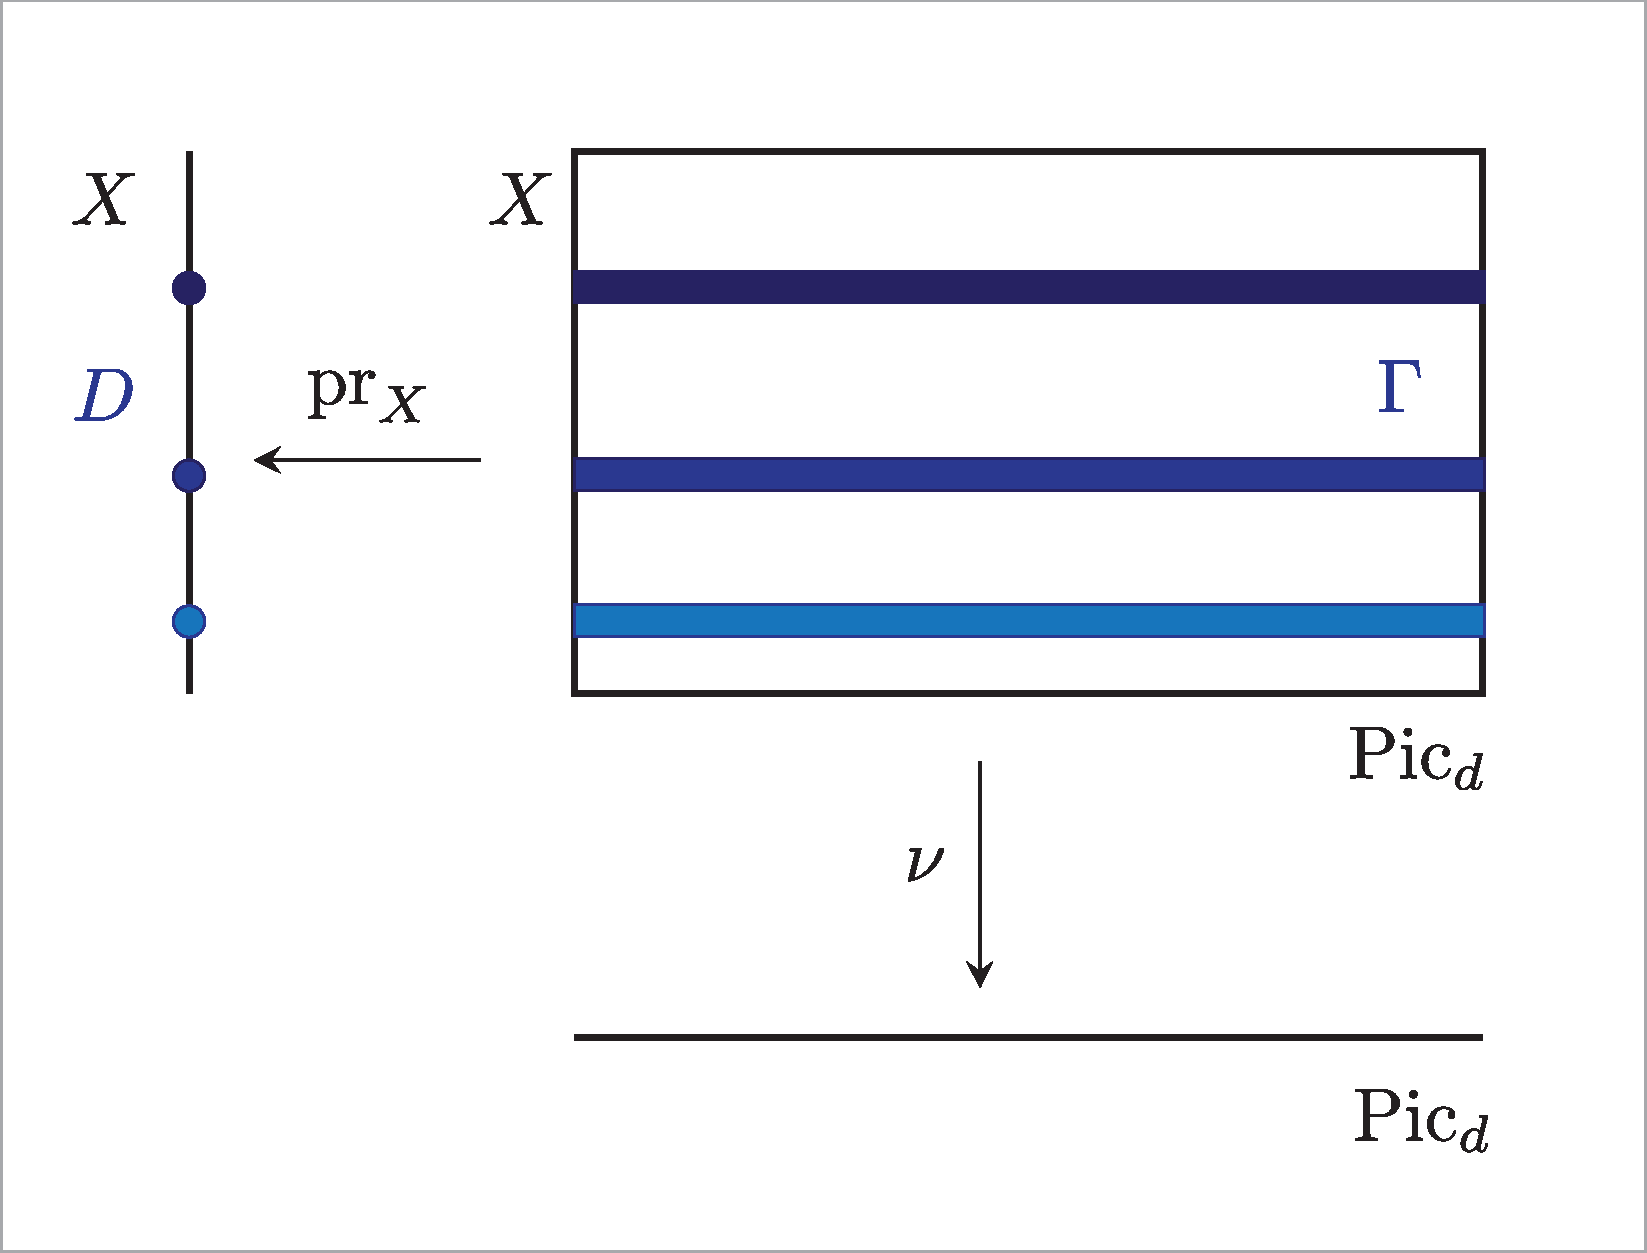
\includegraphics[width=0.85\textwidth]{Locally-free-of-degree-m.pdf}
				\caption{The projection $\nu$ restricts to a finite locally free morphism of degree $m$ on the product $\Gamma\subset X\times \Pd$ }
				\label{fig:locally_free_morphism}
		\end{figure}
		
		\begin{rema}\label{rema:ranks}
			During the proof of the above Lemma we showed that the ranks of the first two bundles appearing in the presentation \eqref{eq:univ_lb_seq} are $d+m-g+1$ and $m$. Keep it in mind, because this fact will be exploited during the proof of the Connectedness Theorem.
		\end{rema}

		Collecting the results of this Chapter, we are now able to write down a commutative diagram in the category of coherent sheaves which is in some sense the \emph{global version} of \eqref{eq:local_diagram} and, thus, gives an identification of the coboundary map $\delta:\pi_* \calO_\Delta(\Delta)\to R^1\pi_*\calO_Z$ with the morphism of locally free sheaves $\Tu:T \Dd\to u^* T \Pd$, representing the tangent map of the \AJJ map $u$ restricted to divisors of degree $d$.

		$$
		\begin{tikzpicture}[node distance=8em, auto]
			%node (O) 									{$0$};
			\node (A) 									{$\pi_* \calO_Z(\Delta)$};
			%node (A2) 	[right of=A]		{$\;$};
			\node (B) 	[right of=A]		{$\pi_* \calO_\Delta(\Delta)$};
			%node (B2) 	[right of=B]		{$\;$};
		  \node (C) 	[right of=B] 	{$R^1 \pi_* \calO_Z$};
			%\node (C2) 	[right of=C] 		{$\;$};
		  \node (D) 	[right of=C] 	{$R^1 \pi_* \calO_Z(\Delta)$};
			%\node (OO) 	[right of=D] 		{$0$};
		  %\node (O') 	[below of=O] 		{$\;$};
		  \node (A') 	[below of=A] 		{$\;$};
		  \node (B') 	[below of=B, yshift=3em] 		{$ T \Dd$};
		  \node (C') 	[below of=C, yshift=3em] 		{$ u^* T \Pd $};
		  \node (D') 	[below of=D] 		{$\;$};
			%\node (OO') [below of=OO] 	{$\;$};
			%\draw[-stealth] 				(O)	to node {} (A);
		  \draw[-stealth]					(A)		to node {} (B);
		  \draw[-stealth]					(B)		to node {$\delta$} (C);
		  \draw[-stealth]					(C)		to node {} (D);
			%\draw[-stealth]					(D)		to node {} (OO);
		  \draw[-stealth]					(B')	to node {$\Tu$} (C');
		  \draw[-stealth][swap]		(B)		to node {$\cong$} (B');
		  \draw[-stealth]					(C)		to node {$\cong$} (C');
		\end{tikzpicture}
		\vspace{-2em}
		$$

		The commutativity of this \emph{global} diagram follows from the commutativity of its fiberwise counterparts -- achieved in Proposition \ref{prop:delta_u} -- together with the fact that the sheaves appearing in the central square are locally free, as we observed in Remark \ref{rema:smoothness}.




